\chapter{Background} \label{chap:background}
This chapter is focused on making the reader familiar with concepts used throughout this report.
First, an introduction to computational complexity is given to establish a mathematical framework to describe the efficiency of computer algorithms.
Second, the basic ideas of quantum mechanics are presented.
Finally, an overview of the quantum computational circuit model is given along with a description of the \acrlong{qft} algorithm and Grover's algorithm.

\section{Computational Complexity}
In computer science, there seems to be a fundamental limit to what problems computers can solve.
Some problems seem to be inherently uncomputable: there exists no general solution that does not go into an infinite loop for certain inputs~\cite{church1936note, turing1937computable}.
This report will not go further into what problems are computable and uncomputable.
Rather, it will look at the computational efficiency of certain algorithms: how many resources are required to solve a problem?

\subsection{Big-O Notation}
The time and space required by an algorithm generally grows as the size of the input grows.
Because of this, it is traditional to describe the efficiency of an algorithm as a function of the size of its input~\cite{cormen2009introduction}.
This function describes the number of primitive operations it performs for a given input size.
The notion of input size here depends on the context of the problem.
For example, when computing the discrete Fourier transform, the input size refers to the dimension of the input vector.
When talking about a problem like integer multiplication, however, it is more fitting to talk about the input size as the number of bits needed to represent the input in binary.

When analyzing the efficiency of algorithms, we look at the asymptotic growth for a given input size.
Consider an algorithm that given input size $n$ takes $n^2$ primitive operations to run and another algorithm that takes $500n^2 + \log n$ primitive operations to run.
In big-O notation, both these algorithms are said to run in $O(n^2)$ time.
That is, the number of primitive operations it performs scales quadratically with the input size.
Constant factors are ignored as they become negligible as $n \to \infty$.
While they are practically significant --- an algorithm that runs in $O(n/2)$ performs half as many primitive operations as an algorithm that runs in $O(n)$ --- they are not relevant to asymptotic analysis. 

Formally, if we have functions $f(n)$ and $g(n)$ such that $f$ eventually grows slower than some multiple of $g$ as $n \to \infty$, we say $f(n) = O(g(n))$.
For example, given $f(n) = 200n^2$ and $g(n) = n^3$, $f$ begins to grow slower than $g$ when $n > 200$.
Thus, $g$ bounds $f$ from above, and $f(n) = O(g(n)) = O(n^3)$.
Some common big-O run times are shown in \Cref{table:common-big-o}, along with their written name and an example.
Throughout this report, algorithms that are bounded above by a polynomial (i.e. all run times until polynomial in \Cref{table:common-big-o}) will be referred to as polynomial-time algorithms, and algorithms that are not bounded above by a polynomial will be referred to as superpolynomial-time algorithms.

\begin{table}[ht]
    \centering
    {\renewcommand{\arraystretch}{1.1}
        \begin{tabular}{ c|c|c }
            Notation & Name & Example \\
            \hline
            $O(1)$ & Constant & Accessing single element from array \\
            $O(\log n)$ & Logarithmic & Binary search \\
            $O(n)$ & Linear & Unstructured database search \\
            $O(n \log n)$ & Linearithmic & Fast Fourier Transform \\
            $O(n^2)$ & Quadratic & Insertion sort \\
            $O(n^k)$ & Polynomial & Gaussian elimination \\
            $O(k^n)$ & Exponential & Graph coloring \\
            $O(n!)$ & Factorial & Brute-force search traveling salesman problem \\
        \end{tabular}
    }
    \caption{Common big-O run times from fast to slow.}
    \label{table:common-big-o}
\end{table}

\subsection{Turing Machines}
The previous section described the measurement of computational efficiency as the number of primitive operations it performs for a given input size.
This abstract definition can be extended by choosing a computational model in order to define what a primitive operation means.
The standard computational model used for this is the Turing machine.
It is chosen as computational model for the analysis of computational efficiency because of its simplicity and because it is able to simulate most physically realizable computational models with little overhead~\cite{arora2009computational}.

A Turing machine is an abstract machine that manipulates symbols from a work alphabet on a finite amount of one-way infinite length tapes divided into cells~\cite{turing1937computable}~(\Cref{fig:single-tape-turing-machine}).
Along these tapes runs a tape head that can read and write one symbol at a time.
The machine has a finite set of states, which the machine executes one at a time by loading them into the state register.
At any time, the machine can be in one of the finite states.
A state can be thought of as a rule with the following form:
\begin{equation} \label{eqn:turing-state}
(q_i,a) \mapsto (q_j,b,H),
\end{equation}
where $q_i$ and $q_j$ are states, $a$ and $b$ are symbols from the work alphabet, and $H \in \{L, S, R\}$ decides how to move the tape head: one cell to the left ($L$), stay in the same position ($S$), or one cell to the right ($R$).
These states as described in \Cref{eqn:turing-state} can be read as ``in state $q_i$, if the read symbol is $a$, go to state $q_j$, write symbol $b$, and move the tape head to $H$."

\begin{figure}[ht]
    \centering
    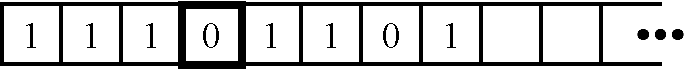
\includegraphics[width=0.5\linewidth]{figures/single-tape-turing-machine.pdf}
    \caption[The tape of a single-tape Turing machine in an arbitrary state.]{The tape of a single-tape Turing machine in an arbitrary state. Note that any multi-tape Turing machines can be efficiently simulated by a single-tape Turing machine~\cite{hartmanis1965computational}, so complexity classes are not affected by changing between single-tape and multi-tape machines.}
    \label{fig:single-tape-turing-machine}
\end{figure}

Everything that can be computed on models of computations we use these days can be computed on a Turing machine~\cite{dershowitz2008natural}.
This hypothesis is known as the Church-Turing thesis.
Related to the Church-Turing thesis is the extended Church-Turing thesis, which states that any physically realizable model of computation can be efficiently simulated on a Turing machine.
That is, can a Turing machine simulate any model of computation in polynomial time?
The quantum computational model brings doubt to this claim.
It is known that quantum computers can efficiently simulate a Turing machine~\cite{bennett1973logical}, but there appears to be no efficient algorithm for simulating a quantum computer on a Turing machine~\cite{deutsch1985quantum}.
Furthermore, \textcite{arute2019quantum} experimentally demonstrated a quantum computer sampling from a probability distribution intractable by a classical computer.
This gives us good reasons to believe that classical computers cannot efficiently simulate quantum computers, and that quantum computers are more computationally powerful for some problems.

\subsection{Complexity Classes}
Complexity classes are sets of computational problems that share some common feature with regard to the computational resources they need to solve some problem~\cite{arora2009computational}.
They are defined in terms of a type of computational problem, computational model, and a bounded resource such as time or space.
In general, most complexity classes describe decision problems solvable by deterministic Turing machines --- though many complexity classes are defined in terms of other types of problems and computational models.
This report mainly focuses on complexity classes involving Turing machines and quantum Turing machines.

The class $\P$ contains all decision problems solvable by a deterministic Turing machine in polynomial time.
Problems that fall under this class are often referred to as tractable or easy problems~\cite{cormen2009introduction}.
The class $\NP$ (non-deterministic polynomial) contains all problems \emph{verifiable} by a deterministic Turing machine in polynomial time.
Equivalently, $\NP$ can be thought of as all problems solvable in polynomial time by a non-deterministic Turing machine.
A non-deterministic Turing machine is a variant of a Turing machine which is not entirely determined by its input and transition function, but can choose from a set of possible transitions when transitioning.
One could then define $\NP$ as consisting of two phases: first, a non-deterministic Turing machine makes a guess about the solution, and then a second, deterministic Turing machine verifies if the guess is correct.
It is clear that $\P \subseteq \NP$, because if you can solve a problem in polynomial time, you can also verify it in polynomial time.
A still unsolved and important question in computer science is whether $\P = \NP$?
That is, can all problems that can be verified in polynomial time also be solved in polynomial time?

In computer science, it is sometimes possible to speed up computation using randomness.
These kinds of algorithms are referred to as probabilistic algorithms and are defined in terms of a probabilistic Turing machine.
A probabilistic Turing machine is a non-deterministic Turing machine that can choose from a set of possible transitions according to some probability distribution when transitioning.
The probabilistic equivalent of $\P$ is $\BPP$ (bounded-error probabilistic polynomial time) and contains all decision problems solvable by a probabilistic Turing machine in polynomial time where a bounded error rate of $1/3$ is allowed.
Since a non-deterministic Turing machine can efficiently simulate a deterministic Turing machine, $\P \subseteq \BPP$.
There are problems to be known in $\BPP$ and not in $\P$, but the number of such problems is decreasing, and \textcite{goldreich2011world, nisan1994hardness} even argue that $\P = \BPP$.

How do quantum computers relate to these complexity classes?
Quantum computers are probabilistic computational devices, and its complexity class equivalent to $\P$ can be defined by replacing the probabilistic Turing machine from $\BPP$ with a quantum computer.\footnote{Note that quantum computers are not simply probabilistic Turing machines as will be shown in the following sections.}
The class $\BQP$ (bounded-error quantum polynomial time) consists all decision problems solvable by a quantum computer in polynomial time where a bounded error rate of $1/3$ is allowed.
It is known that there are $\NP$ problems that can be efficiently solved on a quantum computer like integer factorization, discrete logarithms, and quantum many-body simulation.
As mentioned in the previous section, quantum computers can also solve all problems in $\P$ efficiently, so $\P \subseteq \BQP$.
Furthermore, quantum computers are more powerful than classical probabilistic computers~\cite{bernstein1997quantum}, giving $\BPP \subseteq \BQP$.
How $\BQP$ relates to $\P$ and $\NP$ exactly is still unknown, however, it seems unlikely that $\BQP = \NP$~\cite{aaronson2010bqp}.

\begin{figure}[ht]
    \centering
    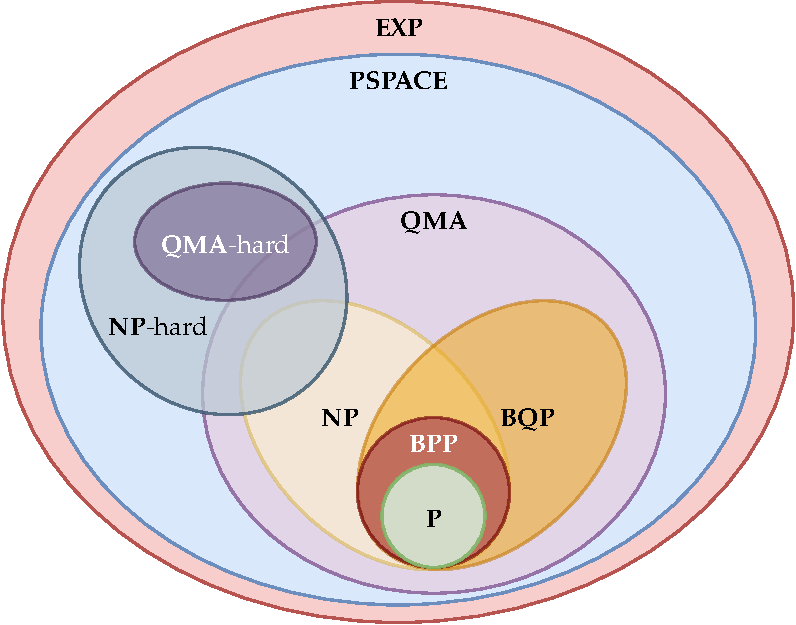
\includegraphics[width=0.4\linewidth]{figures/complexity-classes-hierarchy.pdf}
    \caption[An overview of the hierarchy of the complexity classes discussed.]{An overview of the hierarchy of the complexity classes discussed. This graphic assumes $\P \neq \NP$, $\P \neq \BPP$, and $\P \subseteq \BPP \subseteq \BQP$. $\PSPACE$ is the space equivalent of $\P$, containing all problems that can be solved in polynomial space by a deterministic Turing machine.}
    \label{fig:complexity-classes-hierarchy}
\end{figure}

\section{Quantum Mechanics}
In classic information theory, the smallest unit of information is the bit.
A bit can be in one of two states: 0 or 1.
Quantum information is built upon an analogous concept: the quantum bit, or qubit.
Qubits are physical objects that appear in nature on the scale of atoms and subatomic particles.
A qubit can be any two-state quantum-mechanical system such as the spin of an electron, which can be spin up or down, or the polarization of a photon, which can be horizontally of vertically polarized.
In this report, qubits will be treated as abstract mathematical objects as the physical realization of qubits is beyond the scope of this work.

\subsection{Qubits} \label{sec:quantum-states}
The state of a qubit is denoted as follows:
\begin{equation} \label{eqn:qubit-state}
\ket{\psi} = \alpha_0\ket{0} + \alpha_1\ket{1}.
\end{equation}
Quantum states are often described using Dirac notation \ket{\,\cdotp\,}, which describes a column vector in $\mathbb{C}^{2^n}$.
The states $\{\ket{0}, \ket{1}\}$ are the computational basis states which are defined as $(\begin{matrix}1 & 0\end{matrix})^T$ and $(\begin{matrix}0 & 1\end{matrix})^T$ respectively, and form an orthonormal basis for this vector space.
The values $\alpha, \beta \in \mathbb{C}$ are the state's probability amplitudes, and cannot be examined directly.\footnote{The field of quantum tomography focuses on recovering these values through multiple measurements, but this requires prior knowledge about the system~\cite{d2003quantum}.}
When measuring a qubit, it collapses probabilistically to one of the basis states.
The probability of measuring 0 is given by the absolute square $|\alpha_0|^2$, and the probability of measuring 1 is given by $|\alpha_1|^2$.
As these values are probabilities, they should be normalized: $|\alpha_0|^2 + |\alpha_1|^2 = 1$.
Formally, a qubit can be thought of as a unit vector in a two-dimensional Hilbert space.

A qubit differs from a classical bit in that it can be in a linear combination, or superposition of states.
While a bit can be only be in the state 0 or 1, a qubit can be in one of infinitely many superpositions of states.
However, the laws of quantum mechanics restrict direct access to the probability amplitudes of a state.
Instead, when measuring a qubit, it collapses to basis state \ket{j} with probability $|\alpha_j|^2$.
For example, consider the state
\begin{equation} \label{eqn:plus-state}
\ket{+} = \dfrac{1}{\sqrt{2}}\left(\ket{0} + \ket{1}\right).
\end{equation}
This state has equal probability of measuring 0 and 1, as $|1/\sqrt{2}|^2 = 1/2$.
Note that measurement changes the state of a qubit: if the state from \Cref{eqn:plus-state} is measured as 1, the superposition is lost and the state becomes \ket{1}.

A helpful geometric interpretation of a qubit's state can be obtained by rewriting \Cref{eqn:qubit-state} as
\begin{equation}
\ket{\psi} = e^{i\delta} \left(\cos\dfrac{\theta}{2}\ket{0} + e^{i\varphi}\sin\dfrac{\theta}{2}\ket{1}\right),
\end{equation}
where $\delta, \theta, \varphi \in \mathbb{R}$.
The global phase $e^{i\delta}$ can often be ignored, as $\forall \delta \in \mathbb{R} : |e^{i\delta}| = 1$, so it does not impact measurement outcome~\cite{nielsen2002quantum}.
Simplifying then, the state of a qubit can be written as
\begin{equation}
\ket{\psi} = \cos\dfrac{\theta}{2}\ket{0} + e^{i\varphi}\sin\dfrac{\theta}{2}\ket{1}.
\end{equation}
Here, $\theta$ and $\varphi$ define a point on a three-dimensional sphere referred to as the Bloch sphere (\Cref{fig:bloch-sphere}).
\begin{figure}[ht]
    \centering
    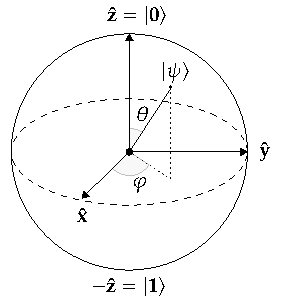
\includegraphics[width=0.365\linewidth]{figures/bloch-sphere.pdf}
    \caption[Bloch sphere representation of a qubit's state.]{Bloch sphere representation of a qubit's state.}
    \label{fig:bloch-sphere}
\end{figure}
While this visualization is limited to a single qubit, it can be a useful visual to build intuition.
For example, the \ket{+} state described in \Cref{eqn:plus-state} can be thought of as being exactly between \ket{0} and \ket{1} on the $x$-axis of the Bloch sphere.

The amount of probability amplitudes grows exponentially with the number of qubits: a $n$-qubit state has $N = 2^n$ amplitudes.
Consider a two-qubit system which lives in a $2^2=4$-dimensional Hilbert space spanned by the computational basis states $\left\{\ket{00}, \ket{01}, \ket{10}, \ket{11}\right\}$.
This state is defined by the linear combination
\begin{equation} \label{eqn:two-qubit-state}
\ket{\psi} = \alpha_0\ket{00} + \alpha_1\ket{01} + \alpha_2\ket{10} + \alpha_3\ket{11}.
\end{equation}
Again, unlike classical bits who can only be in one state at a time, this state can be in a superposition of all four states.
The normalization condition still applies for \Cref{eqn:two-qubit-state}: $\sum_{i=0}|\alpha_i|^2 = 1$.
Single-qubit states can be combined to form multi-qubit states by taking the tensor product of the two states.
Given states $\ket{\psi} = \alpha_0\ket{0} + \alpha_1\ket{1}$ and $\ket{\varphi} = \beta_0\ket{0} + \beta_1\ket{1}$:
\begin{equation} \label{eqn:tensor-product-states}
\begin{aligned}
\ket{\psi} \otimes \ket{\varphi} &= \begin{pmatrix}\alpha_0 \\ \alpha_1\end{pmatrix} \otimes \begin{pmatrix}\beta_0 \\ \beta_1\end{pmatrix} \\
&= \begin{pmatrix}\alpha_0\begin{pmatrix}\beta_0 \\ \beta_1\end{pmatrix} \\ \alpha_1\begin{pmatrix}\beta_0 \\ \beta_1\end{pmatrix}\end{pmatrix} \\
&= \begin{pmatrix}\alpha_0\beta_0 \\ \alpha_0\beta_1 \\ \alpha_1\beta_0 \\ \alpha_1\beta_1\end{pmatrix} \\
&= \alpha_0\beta_0\ket{00} + \alpha_0\beta_1\ket{01} + \alpha_1\beta_0\ket{10} + \alpha_1\beta_1\ket{11}.
\end{aligned}
\end{equation}
Often when describing multi-qubit states, the tensor product will be implied.
The notations
\begin{equation}
\ket{0} \otimes \ket{0} = \ket{0}\ket{0} = \ket{00}
\end{equation}
all describe state.
The relative phases of $\alpha_0, \alpha_1$ and $\beta_0, \beta_1$ in \Cref{eqn:tensor-product-states} are responsible for the quantum mechanical property of interference.
When the phase of $\alpha_j$ and $\beta_k$ is the same, they will interfere constructively and increase the probability amplitude for that state.
On the other hand, if $\alpha_j$ and $\beta_k$ have opposite phases, they will interfere destructively and decrease the probability amplitude for that state.

Not all multi-qubit systems can be expressed as a tensor product of individual states as shown in \Cref{eqn:tensor-product-states}.
Consider the following state:
\begin{equation} \label{eqn:bell-state}
\ket{\Phi^+} = \dfrac{1}{\sqrt{2}}\left(\ket{00} + \ket{11}\right).
\end{equation}
This state cannot be expressed as a tensor product of two individual states, as that would imply $\big(\alpha_0\beta_0 = \alpha_1\beta_1 = 1/\sqrt2\,\big) \wedge \big(\alpha_0\beta_1 = \alpha_1\beta_0 = 0\big)$, which is a contradiction.
States like $\ket{\Phi^+}$ are referred to as entangled states.
Entanglement is the quantum phenomena of correlation in measurement outcomes.
For example, when measuring the state $\ket{\Phi^+}$ from \Cref{eqn:bell-state}, the only two possible measurement outcomes are 00 and 11.
So by measuring one qubit, one also knows the state of the other qubit.

\subsection{State Evolution} \label{sec:state-evolution}
The evolution of a closed quantum system is described by a unitary transformation~\cite{nielsen2002quantum}.\footnote{In this report, a perfectly closed system is assumed, even though in reality all systems interact somewhat with other systems.}
A state \ket{\psi} at time $t_1$ is related to state \ket{\psi'} at time $t_2$ by a unitary operator $U$:
\begin{equation}
\ket{\psi'} = U\ket{\psi}.
\end{equation}
The unitary nature of these operators implies $UU^\dagger = U^\dagger U = I$, where $^\dagger$ is the conjugate transpose and $I$ the identity matrix.
Single-qubit operators can be represented as $2 \times 2$ complex-valued unitary matrices.
A common single-qubit operator is the Pauli-$X$ operator which transforms a state $\alpha_0\ket{0} + \alpha_1\ket{1}$ to $\alpha_1\ket{0} + \alpha_0\ket{1}$.
It is part of the set of Pauli matrices:
\begin{equation}
X = \xgate{}, \hspace*{5mm}
Y = \ygate{}, \hspace*{5mm}
Z = \zgate{}.
\end{equation}
These matrices are ubiquitous in the study of quantum computation and information.
Another useful and common operator is the Hadamard operator:
\begin{equation}
H = \hgate{},
\end{equation}
which maps the computational basis states to an equal superposition state.

The Pauli-$Z$ operator is part of the $Z$-rotation operators family.
The general form for $Z$-axis rotation can be described as follows:
\begin{equation}
R_z(\theta) = \phasegate{}.
\end{equation}
From this definition follows that $Z = R_z(\pi)$.
Other common $Z$-axis rotation operators are $S = R_z(\pi/2)$ and $T = R_z(\pi/4)$.
Note that all $Z$-axis rotation operators only influence the \ket{1} amplitude of the state:
\begin{equation}
\begin{aligned}
R_z(\theta)\ket{0} &= \ket{0} \\
R_z(\theta)\ket{1} &= e^{i\theta}\ket{1}.
\end{aligned}
\end{equation}

Multi-qubit operators act on two or more qubits and are required for creating entangled states.
Two common two-qubit operators are the $\textnormal{CNOT}$ and $CZ$ operators.
The $\textnormal{CNOT}$ operator can be thought of as a controlled-$X$ operator, which applies an $X$ operation on the target qubit if the control qubit is in the \ket{1} state.
Equivalently, the $CZ$ operator applies a $Z$ operation on the target qubit if the control qubit is \ket{1}.
Their matrix representations are as follows:
\begin{equation}
\textnormal{CNOT} = \cnotgate{}, \hspace*{5mm}
CZ = \czgate{}.
\end{equation}
Generally, a controlled-$U$ operator applies $U$ on the target qubit if the control qubit is \ket{1}.

\subsection{Measurement}
While the evolution of quantum states in a closed system is unitary, at some point the quantum state has to interact with the outside world.
This is what measurement means: any interaction from an outside system with the quantum system.
Formally, measurement is defined by a set of measurement operators  $\{M_m\}$, where the probability of measuring the state $m$ is given by
\begin{equation}
p(m) = \bra{\psi}M_m^\dagger M_m\ket{\psi}.
\end{equation}
With $\bra{\psi} = \ket{\psi}^\dagger$, this equation can then be read as the inner product between $M_m\ket{\psi}$ and itself. 
This is just a generalization of the definition of measurement given in \Cref{sec:quantum-states}.
For example, what is the probability of measuring 0 for an arbitrary state $\ket{\psi} = \alpha_0\ket{0} + \alpha_1\ket{1}$?
Using $M_0 = \op{0}{0}$:
\begin{equation} \label{eqn:measurement}
\begin{aligned} 
p(0) &= \bra{\psi}M_0^\dagger M_0\ket{\psi} \\
&= \ip{\psi}{0}\ip{0}{0}\ip{0}{\psi} \\
&= \ip{\psi}{0}\ip{0}{\psi} \\
&= \begin{pmatrix}\alpha_0^* & \alpha_1^*\end{pmatrix}\begin{pmatrix}1 \\ 0\end{pmatrix}
\begin{pmatrix}1 & 0\end{pmatrix}\begin{pmatrix}\alpha_0 \\ \alpha_1\end{pmatrix} \\
&= \alpha_0^* \alpha_0 \\
&= |\alpha_0|^2.
\end{aligned}
\end{equation}
Similarly, using $M_1 = \op{1}{1}$ gives $p(1) = |\alpha_1|^2$.
Measuring with the measurement operators $\left\{\op{0}{0}, \op{1}{1}\right\}$ is referred to as measuring in the computational basis.

After measurement, the state of the system can be described as follows:
\begin{equation}
\ket{\psi} = \dfrac{M_m\ket{\psi}}{\sqrt{p(m)}}.
\end{equation}
Following the example from \Cref{eqn:measurement} with $M_0 = \op{0}{0}$ and $p(0) = |\alpha_0|^2$, after measuring 0 the system is in the state
\begin{equation}
\begin{aligned}
\ket{\psi} &= \dfrac{\ket{0}\ip{0}{\psi}}{\sqrt{|\alpha_0|^2}} \\
&= \dfrac{\ket{0}\alpha_0}{|\alpha_0|} \\
&= \dfrac{\alpha_0}{|\alpha_0|} \ket{0}.
\end{aligned}
\end{equation}
Note that a global phase $e^{i\delta}$ shows up as the factor $\alpha_0/|\alpha_0|$.
As mentioned in \Cref{sec:quantum-states}, the states $e^{i\delta}\ket{0}$ and $\ket{0}$ are considered equal up to the global phase factor.

A special class of measurements called projective measurements can sometimes be used to simplify calculations.
A projective measurement is defined by an observable $O$, which is a Hermitian operator on the state space of the system.
This observable has a spectral decomposition
\begin{equation}
O = \sum_{\lambda}\lambda P_\lambda,
\end{equation}
where $P_\lambda$ is the projector onto the eigenspace of $O$ with eigenvalue $\lambda$.
For example, the Pauli-$Z$ operator can be thought of as an observable with the spectral decomposition
\begin{equation}
Z = 1\op{0}{0} - 1\op{1}{1},
\end{equation}
which has eigenvectors $\{\ket{0}, \ket{1}\}$ with respective eigenvalues $\{1, -1\}$.
As the observable $Z$ has the computational basis states as eigenvectors, a measurement of $Z$ can also be thought of a measuring in the computational basis.
With this definition of projective measurements, the expectation value of an observable $O$ for state \ket{\psi} can be defined as
\begin{equation}
\begin{aligned}
\expval{O}_\psi &= \bra{\psi}O\ket{\psi} \\
&= \big(\alpha_0^*\bra{\lambda_0} + \ldots + \alpha_{N-1}^*\bra{\lambda_{N-1}}\big) \big(\alpha_0O\ket{\lambda_0} + \ldots + \alpha_{N-1}O\ket{\lambda_{N-1}}\big) \\
&= \big(\alpha_0^*\bra{\lambda_0} + \ldots + \alpha_{N-1}^*\bra{\lambda_{N-1}}\big) \big(\alpha_0\lambda_0\ket{\lambda_0} + \ldots + \alpha_{N-1}\lambda_{N-1}\ket{\lambda_{N-1}}\big) \\
&=  \left\lvert \alpha_0\right\rvert^2\lambda_0 + \ldots + \left\lvert \alpha_{N-1}\right\rvert^2 \lambda_{N-1} \\
&= \sum_{i=0}^{N-1} \left\lvert \alpha_i\right\rvert^2\lambda_i.
\end{aligned}
\end{equation}
The expectation value is the sum of all possible outcomes (eigenvalues of $O$) weighted by their probability.
Calculating the expectation value experimentally means preparing and measuring the state multiple times and is a practically useful notation to describe the behavior and output of quantum computations.

\section{Quantum Computation}
This section combines the theory of computer science and quantum mechanics to introduce the fundamental model of quantum computation: the quantum circuit model.

\subsection{Quantum Circuits}
Analogous to the classical circuit model, the quantum circuit model uses gates which act on data.
In the classical circuit model boolean functions (logic gates) act on bits, while in the quantum circuit model quantum gates act on qubits.
Most of the common quantum gates used in quantum computing were already described as operators in \Cref{sec:state-evolution}.
To be more in line with the nomenclature of classical computing, from here on out these operators will be referred to as quantum gates in the context of quantum circuits.

In a quantum circuit time moves from left to right, where qubits are represented by wires on which gates can act, and classical bits are represented by double-lined wires.
Usually the qubits are assumed to be instantiated to \ket{0}, unless noted otherwise.
A list of frequently used quantum gates is shown in \Cref{table:common-quantum-gates}.
Quantum gates are unitary and thus reversible, making the quantum circuit model a reversible model of computation.
The inverse of a gate $U$ is denoted as the conjugate transpose $U^\dagger$.
By the definition of unitary $UU^\dagger = U^\dagger U = I$, applying the inverse $U^\dagger$ after $U$ essentially uncomputes $U$ and vice versa.
Gates whose conjugate transpose are equal to themselves are referred to as Hermitian.
For example, $H$ is Hermitian as $H^\dagger = H$ and thus $H^2 = I$.
 
\Cref{fig:bell-state-circuit} demonstrates a simple quantum circuit which creates the maximally entangled state $\ket{\Phi^+} = \left(\ket{00} + \ket{11}\right)/\sqrt{2}$ from \Cref{eqn:bell-state} and measures both qubits.
This state is one of four maximally entangled two-qubit states referred to as a Bell state.
\begin{figure}[ht]
    \Large
    \[
    \Qcircuit @C=1em @R=0.7em @!R {
        \push{\rule{0em}{1em}} & & \lstick{\ket{0}} & \gate{H} & \ctrl{1} & \meter & \cw  \\
        \push{\rule{0em}{1em}} & & \lstick{\ket{0}} & \qw & \targ & \meter & \cw \\
    }
    \]
    \caption{Quantum circuit for creating and measuring a Bell state \ket{\Phi^+}.}
    \label{fig:bell-state-circuit}
\end{figure}
This circuit does the following.
The system starts in state $\ket{\psi} = \ket{00}$.
A Hadamard gate is applied on the first (using least-significant bit order) qubit:
\begin{align}
\ket{\psi} &= \ket{0}\dfrac{1}{\sqrt{2}}\left(\ket{0} + \ket{1}\right) \\
&= \dfrac{1}{\sqrt{2}}\left(\ket{00} + \ket{01}\right).
\end{align}
Then, a $\textnormal{CNOT}$ is applied with the first qubit as control and the second qubit as target, giving the final state
\begin{equation}
\ket{\psi} = \dfrac{1}{\sqrt{2}}\left(\ket{00} + \ket{11}\right).
\end{equation}
This state is then measured, which will measure 00 or 11 with equal probability.

\begin{table}[ht]
    \centering
    {\renewcommand{\arraystretch}{1.1}
        \begin{tabular}{ c|c|c }
            Gate name & Circuit symbol & Matrix representation \\
            \hline
            Hadamard &
            \Large
            \Qcircuit @C=1em @R=1em @!R {
                & \gate{H} & \qw
            }
             & $\hgate{}$ \\
             Pauli-$X$ &
             \Large
             \Qcircuit @C=1em @R=1em @!R {
                 & \gate{X} & \qw
             }
             & $\xgate{}$ \\
             Pauli-$Y$ &
             \Large
             \Qcircuit @C=1em @R=1em @!R {
                 & \gate{Y} & \qw
             }
             & $\ygate{}$ \\
             Pauli-$Z$ &
             \Large
             \Qcircuit @C=1em @R=1em @!R {
                 & \gate{Z} & \qw
             }
             & $\zgate{}$ \\
             Phase ($S$) &
             \Large
             \Qcircuit @C=1em @R=1em @!R {
                 & \gate{S} & \qw
             }
             &
             $\begin{pmatrix}1 & 0 \\ 0 & i\end{pmatrix}$ \\
             $T$ &
             \Large
             \Qcircuit @C=1em @R=1em @!R {
                 & \gate{T} & \qw
             }
             &
             $\begin{pmatrix}1 & 0 \\ 0 & e^{i\pi/4}\end{pmatrix}$ \\
             $\textnormal{CNOT}$ &
             $
             \Large
             \Qcircuit @C=1em @R=1em {
                 & \ctrl{1} & \qw \\
                 & \targ & \qw
             }
             $
             & $\cnotgate{}$ \\
             $CZ$ &
             $
             \Large
             \Qcircuit @C=1em @R=1em {
                 & \ctrl{1} & \qw \\
                 & \control \qw & \qw
             }
             $
             & $\czgate{}$ \\
        \end{tabular}
    }
    \caption{Frequently used quantum gates and circuit symbols.}
    \label{table:common-quantum-gates}
\end{table}

In classical computations, copying bits is a common operation.
However, in quantum computing the data one can copy is much more restricted.
If a qubit is in a computational basic state, that state can be copied by a $\textnormal{CNOT}$ gate~(\Cref{fig:copy-basis-state}).
\begin{figure}[ht]
    \Large
    \[
    \Qcircuit @C=1em @R=0.7em @!R {
        \push{\rule{0em}{1em}} & & \lstick{\ket{j}} & \ctrl{1} & \qw & \ket{j}  \\
        \push{\rule{0em}{1em}} & & \lstick{\ket{0}} & \targ & \qw & \ket{j} \\
    }
    \]
    \caption{Copying a computational basis state using $\textnormal{CNOT}$ where $j \in \{0, 1\}$.}
    \label{fig:copy-basis-state}
\end{figure}
However, trying to copy an arbitrary state $\ket{\psi} = \alpha_0\ket{0} + \alpha_1\ket{1}$ using the circuit in \Cref{fig:copy-basis-state} gives
\begin{equation}
\ket{\psi} = \alpha_0\ket{00} + \alpha_1\ket{11}.
\end{equation}
This state does not contain two copies of \ket{\psi} (unless $\alpha_0\alpha_1 = 0$ as is true with computational basis states), which should have the form
\begin{equation}
\ket{\psi}\ket{\psi} = \alpha_0^2\ket{00} + \alpha_0\alpha_1\ket{01} + \alpha_1\alpha_0\ket{10} + \alpha_1^2\ket{11}.
\end{equation}
In fact, is it impossible to copy an unknown quantum state.
There exists no solution for a unitary operator $U$ that does the transformation
\begin{equation}
\alpha_0\ket{00} + \alpha_1\ket{01} \xrightarrow[]{U} \alpha_0^2\ket{00} + \alpha_0\alpha_1\ket{01} + \alpha_1\alpha_0\ket{10} + \alpha_1^2\ket{11}.
\end{equation}
This property is known as the no-cloning theorem, and is a fundamental limit of quantum information.
Note that this holds for unknown quantum states.
If one has the circuit to prepare \ket{\psi}, you could simply create \ket{\psi}\ket{\psi} by executing the circuit on a second qubit.

\subsection{Universal Gate Sets}
A universal gate set is defined as a finite set of gates that can be used to represent any other gate.
In the classical circuit model, \textsc{NAND} is a universal gate with which all other gates can be represented.
Equivalently, universal quantum gate sets are sets of quantum gates to which any quantum operation can be reduced to.
A common universal gate set is $\{\textnormal{CNOT}, H, S, T\}$.
Any quantum operation can be reduced to a combination of $\textnormal{CNOT}, H, S$ and  $T$ gates.
For example, the three-qubit equivalent of the \textnormal{CNOT} gate, the Toffoli gate, can be decomposed into these gates as shown in~\Cref{fig:decomposition-toffoli}.
\begin{figure}[H]
    \Large
    \[
    \Qcircuit @C=0.6em @R=0.7em @!R {
        & \ctrl{1} & \qw   & &   & \qw      & \qw      & \qw              & \ctrl{2} & \qw & \qw & \qw & \ctrl{2} & \qw & \ctrl{1} & \qw & \ctrl{1} & \gate{T} & \qw \\
        & \ctrl{1} & \qw   & = & & \qw      & \ctrl{1} & \qw              & \qw   & \qw &        \ctrl{1} & \qw & \qw & \gate{T^\dagger} & \targ & \gate{T^\dagger} & \targ & \gate{S} & \qw \\
        & \targ \qwx & \qw & & & \gate{H} & \targ      & \gate{T^\dagger} & \targ & \gate{T} & \targ & \gate{T^\dagger} & \targ & \gate{T} & \gate{H} & \qw & \qw & \qw & \qw
    }
    \]
    \caption{Decomposition of the Toffoli gate using $\textnormal{CNOT}, H, S$ and $T$ gates.}
    \label{fig:decomposition-toffoli}
\end{figure}

\subsection{Quantum Algorithms}
To demonstrate the quantum circuit computational model's ability to solve certain problems more efficiently than classical computers, two quantum algorithms which provide a speedup over their classical counterparts are now reviewed: the \acrfull{qft} and Grover's algorithm.

\subsubsection{Quantum Fourier Transform}
The \gls{qft} is the quantum analogue of the \emph{inverse} \gls{dft}.
The \gls{dft} is ubiquitous in the fields of engineering and computer science.
In short, it transforms a signal in the time domain to the frequency domain, and vice versa with the inverse \gls{dft}.
For $N = 2^n$ amplitudes, the \gls{qft} uses $O(n^2)$ gates, where $n$ is the amount of qubits.
The best-known classical algorithm for computing the \gls{dft} uses $O(n2^n)$ gates.
That is, the \gls{qft} is exponentially more efficient than the best-known classical algorithm.
However, the applications of the \gls{qft} are limited.
The result of the \gls{qft} are stored in the amplitudes of the quantum state.
These amplitudes cannot be directly accessed by measurement, so there is no way to extract the results.
On the other hand, the \gls{qft} is the backbone of the phase estimation algorithm, which in term can be used to solve problems including the order-finding problem and the factoring problem efficiently.

The inverse \gls{dft} is a linear transformation on an input vector of $N$ complex values $(\begin{matrix}x,\ldots,x_N\end{matrix})$.
It transforms a element $x_k$ as follows:
\begin{equation}
x_k' = \dfrac{1}{\sqrt{N}} \sum_{j=0}^{N-1} x_j e^{\tfrac{2\pi i}{N}jk}.
\end{equation}
Equivalently, the \gls{qft} is defined as a unitary operator which acts on a computational basis state \ket{j} as following:
\begin{equation}
\ket{j} \rightarrow \dfrac{1}{\sqrt N}\sum_{k=0}^{N-1}e^{\tfrac{2\pi i}{N} jk}\ket{k}.
\end{equation}
To describe the quantum circuit for the \gls{qft}, the following definition is useful:
\begin{equation}
R_k = \begin{pmatrix}
1 & 0 \\
0 & e^{\tfrac{2\pi i}{2^k}}
\end{pmatrix}.
\end{equation}
Some useful identities are $R_2 = S$ and $R_3 = T$.
Using this gate, the general quantum circuit for the \gls{qft} is shown in \Cref{fig:qft-general-circuit}.
The gates at the end of the circuit are swap gates, which swaps two qubits.
This is necessary to get the result in the correct order.

\begin{figure}[ht]
    \begin{adjustwidth}{-1cm}{-1cm}
        \[
        \Qcircuit @C=0.7em @R=0.5em @!R {
            & \push{\rule{0em}{1em}} & & \lstick{\ket{j_1}} & \gate{H} & \gate{R_2} & \qw & \dots & & \gate{R_{n-1}} & \gate{R_n} & \qw & \qw & \qw & \qw & \qw & \qw & \qw & \qw & \qw & \qw & \qw & \qw & \qw & \qswap \qwx[4] & \qw & \qw \\
            & \push{\rule{0em}{1em}} & & \lstick{\ket{j_2}} & \qw & \ctrl{-1} & \qw & \dots & & \qw & \qw & \gate{H} & \qw & \dots & & \gate{R_{n-2}} & \gate{R_{n-1}} & \qw & \dots & & \qw & \qw & \qw & \qw & \qw & \qswap \qwx[2] & \qw \\
            & \vdots & & & & \vdots & & & & & & & & & & & & & & & & & \vdots \\
            & \push{\rule{0em}{1em}} & & \lstick{\ket{j_{n - 1}}} & \qw & \qw & \qw & \qw & \qw & \ctrl{-3} & \qw & \qw & \qw & \qw & \qw & \ctrl{-2} & \qw & \qw & \dots & & \gate{H} & \gate{R_2} & \qw & \qw & \qw & \qswap & \qw \\
            & \push{\rule{0em}{1em}} & & \lstick{\ket{j_n}} & \qw  & \qw & \qw & \qw & \qw & \qw & \ctrl{-4} & \qw & \qw & \qw & \qw & \qw & \ctrl{-3} & \qw & \dots & & \qw & \ctrl{-1} & \gate{H} & \qw & \qswap & \qw & \qw \\
        }
        \]
    \end{adjustwidth}
    \caption{The general circuit for the \acrshort{qft} on $2^n$ amplitudes with $n$ qubits.}
    \label{fig:qft-general-circuit}
\end{figure}

The \gls{qft} circuit works as follows.
With $N = 2^n$ where $n$ is the number of qubits, the computational basis exists of the states $\left\{\ket{0}, \ldots, \ket{N-1}\right\}$.
We use the notation $\ket{j}$ for a decimal number $j$ in the binary representation $j_1,\ldots,j_n$, e.g. $\ket{15} = \ket{j_1j_2j_3j_4} = \ket{1111}$.
Furthermore, the following notation is used to represent fractional binary numbers:
\begin{equation}
[0.j_1\ldots j_m] = \sum_{k=1}^{m} j_k2^{-k}.
\end{equation}
For example, $j_1/2 + j_2/2^2$ is written as $[0.j_1j_2]$ in fractional binary notation.
Using these definitions, the \gls{qft} can be represented as follows:
\begin{equation}
\textnormal{QFT}\ket{j_1 \ldots j_n} = \dfrac{1}{\sqrt{N}}\left(\ket{0} + e^{2\pi i [0.j_n]}\ket{1}\right)\left(\ket{0} + e^{2\pi i [0.j_{n-1}j_n]}\ket{1}\right)\cdots\left(\ket{0} + e^{2\pi i [0.j_1j_2\ldots j_n]}\ket{1}\right).
\end{equation}
The transformed values end up in the relative phases of the amplitudes.
Again, these relative phases cannot be extracted, but the \gls{qft} is an essential part of many important quantum algorithms.

\subsubsection{Grover's Algorithm}
Grover's algorithm is a quantum algorithm for unstructured database search.
Suppose you want to search through a search space of $n$ numbers.
Given a function $f(x)$ that returns $1$ for the number $\omega$ that you are looking for, and $0$ for every other number:
\begin{equation} \label{eqn:black-box-fn}
f(x) =
\begin{cases}
\begin{aligned}
1 & \text{ if } x = \omega \\
0 & \text{ if } x \neq \omega
\end{aligned}
\end{cases}
\end{equation}
The goal is to find a $x$ so that $f(x) = 1$.
On a classical computer, the best we can do is an exhaustive search of the entire search space, which takes $O(n)$ function calls.
Using a quantum computer, this can be done with $O(\sqrt{n})$ function calls using Grover's algorithm~\cite{grover1996fast}.
Grover's algorithm is asymptotically optimal: \textcite{zalka1999grover} show that $O(\sqrt{n})$ is the best we can do for unstructured database search.

A common problem in computer science is examining a large number of different possibilities to see which of them satisfy a given condition.
This is the same problem that Grover's algorithm looks to solve.
Usually, there is some structure in the problem which allows for more efficient algorithms.
For example, if a list of numbers is sorted, one can find a number in $O(\log n)$ using binary search.
For hard problems that do not have such obvious structure like the boolean satisfiability problem, Grover's algorithm can provide a quadratic speedup.

The function $f(x)$ from \Cref{eqn:black-box-fn} is sometimes referred to as a black box function, as its internal workings is not of interest.
Grover's algorithm is a general algorithm which can be applied to many algorithms that use search heuristics.
The quantum equivalent of a black box function is called an oracle, and has the following form:
\begin{equation} \label{eqn:oracle}
U_\omega\ket{x} = 
\begin{cases}
\begin{aligned}
-\ket{x} & \text{ if } x = \omega \\
\phantom{-}\ket{x} & \text{ if } x \neq \omega
\end{aligned}
\end{cases}
\end{equation}
where \ket{x} is any computational basis state, and $\omega$ is the bit string to find.
That is, it marks the solution to the search problem by shifting the phase of the solution.
An oracle \Cref{eqn:oracle} can be defined in terms of a black box function:
\begin{equation}
U_\omega\ket{x} = (-1)^{f(x)}\ket{x},
\end{equation}
which has the following matrix representation:
\begin{equation}
U_\omega =
\begin{pmatrix}
(-1)^{f(0)} & 0 & \cdots & 0 \\
0 & (-1)^{f(1)} & \cdots & 0 \\
\vdots & 0 & \ddots & \vdots \\
0 & 0 & \cdots & (-1)^{f(2^n-1)}
\end{pmatrix}.
\end{equation}
With the oracle defined, the quantum circuit of Grover's algorithm is shown in \Cref{fig:grover-circuit}.
The qubits can be thought of as being in two registers: the target qubits $\ket{q1\ldots q_n}$ and the oracle qubit \ket{y}.
The oracle qubit \ket{y} starts in the state $H\ket{1} = (\ket{0} - \ket{1})/\sqrt{2}$.
When the oracle is applied to $\ket{q1\ldots q_n}(\ket{0} - \ket{1})/\sqrt{2}$ and $x$ is not a solution, the state stays the same.
However, if the oracle is applied to $\ket{q1\ldots q_n}(\ket{0} - \ket{1})/\sqrt{2}$ and $x$ \emph{is} a solution, the state becomes $-\ket{q1\ldots q_n}(\ket{0} - \ket{1})/\sqrt{2}$.
After the oracle is applied, the solution is marked with a negative phase.
To extract this solution, a procedure called amplitude amplification is used.

\begin{figure}[ht]
    \[
    \Large
    \Qcircuit @C=1em @R=0.5em @!R {
        \push{\rule{0em}{1em}} & & & & \lstick{\ket{q_1} = \ket{0}} & \gate{H} & \multigate{3}{U_\omega} & \gate{H} & \multigate{2}{2\op{0^n}{0^n} - I} & \gate{H} & \meter & \cw \\
        & & \rstick{\,\vdots} & & & & & & & & \vdots \\
        \push{\rule{0em}{1em}} & & & & \lstick{\ket{q_n} = \ket{0}} & \gate{H} & \ghost{U_\omega} & \gate{H} & \ghost{2\op{0^n}{0^n} - I} & \gate{H} & \meter & \cw \\
        \push{\rule{0em}{1em}} & & & & \lstick{\ket{y} = \ket{1}} & \gate{H} & \ghost{U_\omega} &  \qw & \qw \gategroup{1}{7}{4}{10}{1em}{--} & \qw & \qw & \qw \\
        & & & & & & & \hspace{4cm} O(\sqrt{N}) \mbox{ times}
    }
    \]
    \caption{Quantum circuit representation of Grover's algorithm.}
    \label{fig:grover-circuit}
\end{figure}

\noindent
Amplitude amplification can be thought of as inversion about the mean.
Consider a search space of $N = 4$ with two qubits where we are looking for $\omega = 10$.
The amplitudes of the search space start out in an equal superposition:
\begin{figure}[ht]
    \centering
    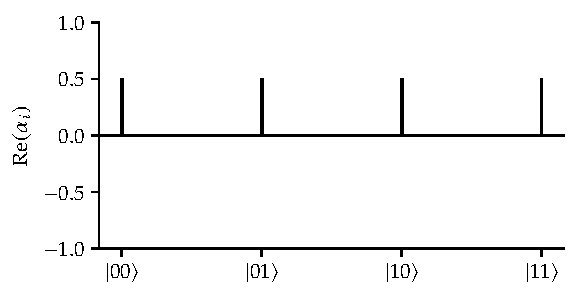
\includegraphics[width=0.5\linewidth]{figures/aa_initial_equal.pdf}
\end{figure}

\noindent
After applying the oracle $U_\omega$ the solution state \ket{10} has its phase flipped:
\begin{figure}[ht]
    \centering
    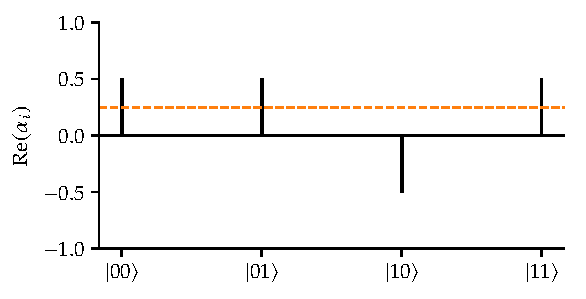
\includegraphics[width=0.5\linewidth]{figures/aa_phase_flipped_mean.pdf}
\end{figure}

\noindent
Note that measuring this state will still give each state with equal probabilities.
Using the diffusion operator $H^{\otimes n}\left(2\op{0^n}{0^n} - I\right)H^{\otimes n}$, the amplitudes are inverted about their mean (displayed as the dotted orange line):
\begin{figure}[ht]
    \centering
    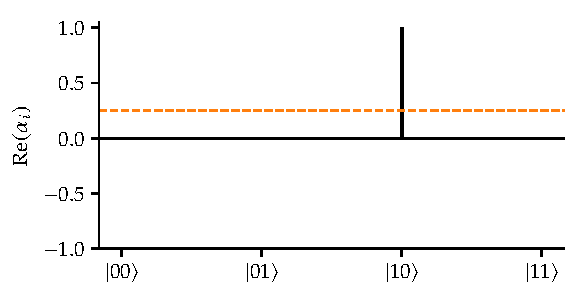
\includegraphics[width=0.5\linewidth]{figures/aa_diffused.pdf}
\end{figure}

\noindent
The application of the oracle and amplitude amplification is often referred to as a Grover iteration.
For this example, one Grover iteration was enough to give a probability of 1 of measuring the correct solution.
Generally, the upper bound on the number of iterations  $R$ required is as follows:
\begin{equation}
R \leq \left\lceil \dfrac{\pi}{4}\sqrt{\dfrac{M}{N}} \right\rceil,
\end{equation}
where $M$ is the number of solutions and $N = 2^n$ is the size of the search space.